% \Image{Capa do livro (; )}{PNLD2022-010-01.png}

% \Image{Ilustração do livro (; )}{PNLD2022-010-04.png}
% \Image{Ilustração do livro (; )}{PNLD2022-010-05.png}
% \Image{Ilustração do livro (; )}{PNLD2022-010-06.png}


\documentclass[11pt]{extarticle}
\usepackage{manualdoprofessor}
\usepackage{fichatecnica}
\usepackage{lipsum,media9}
\usepackage[justification=raggedright]{caption}
\usepackage[one]{bncc}
\usepackage[hedra]{../edlab}
\usepackage{marginnote}
\usepackage{pdfpages}
\usepackage[printwatermark]{xwatermark}
\newwatermark[pagex=2]{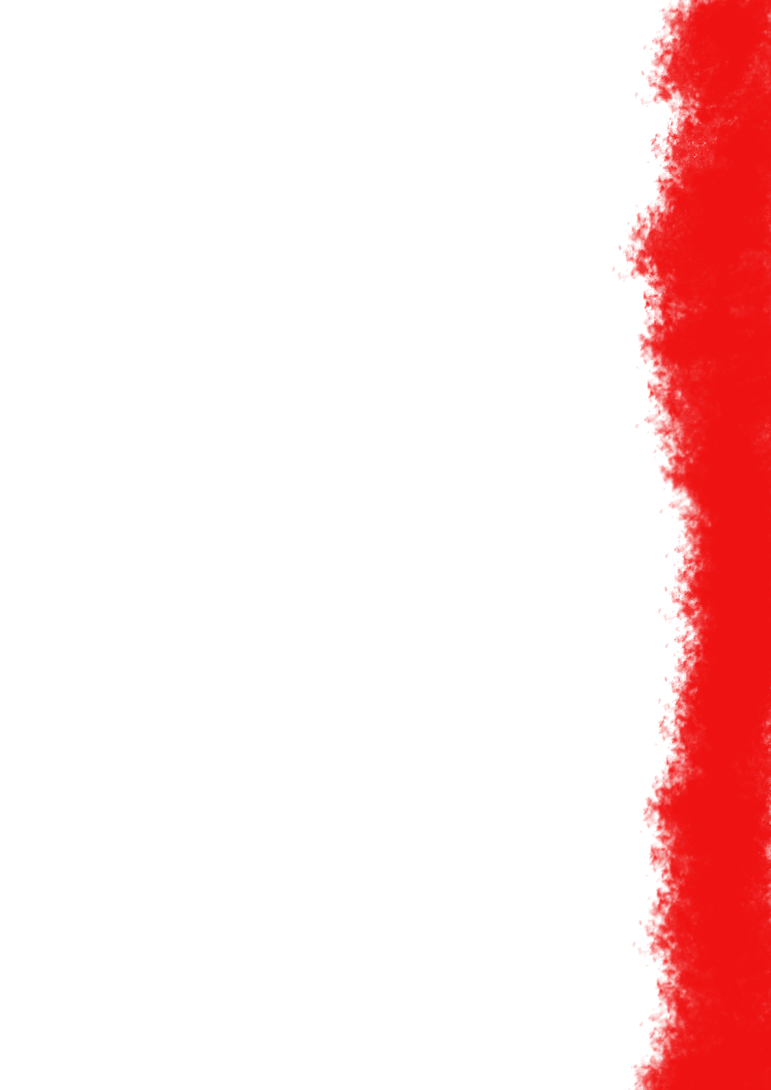
\includegraphics[scale=3.3]{watermarks/test-a.png}}	% página específica
%\newwatermark[oddpages]{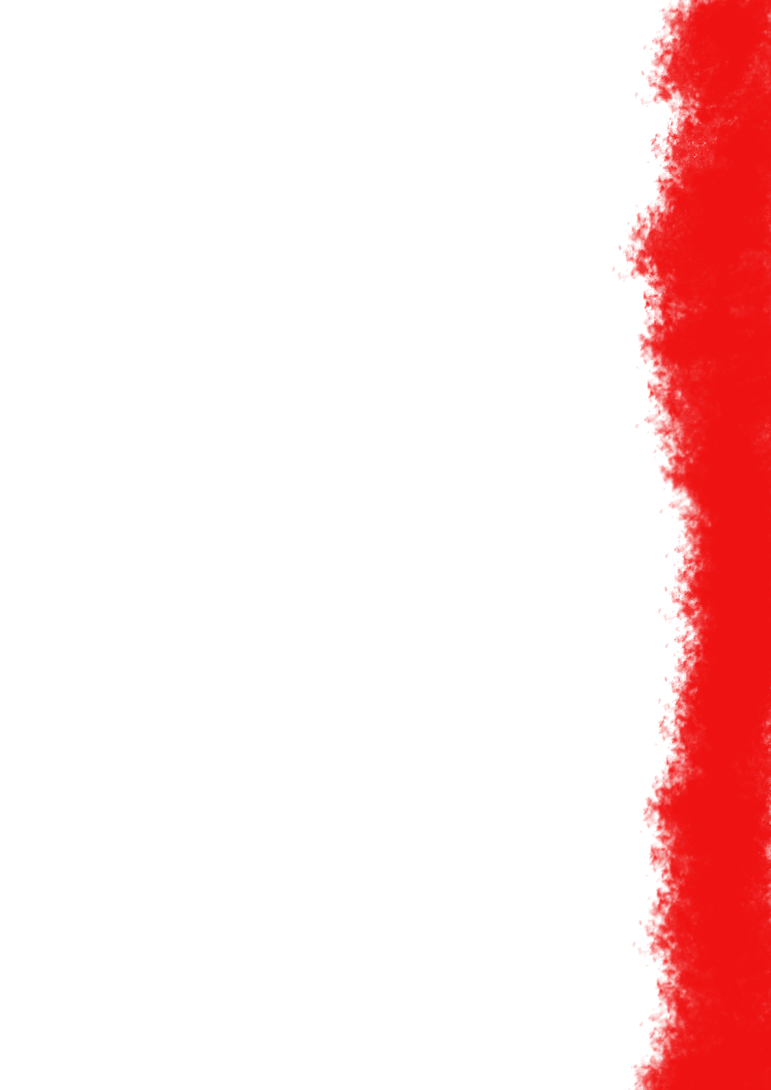
\includegraphics{watermarks/test-a.png}}			% páginas ímpars
%\newwatermark[evenpages]{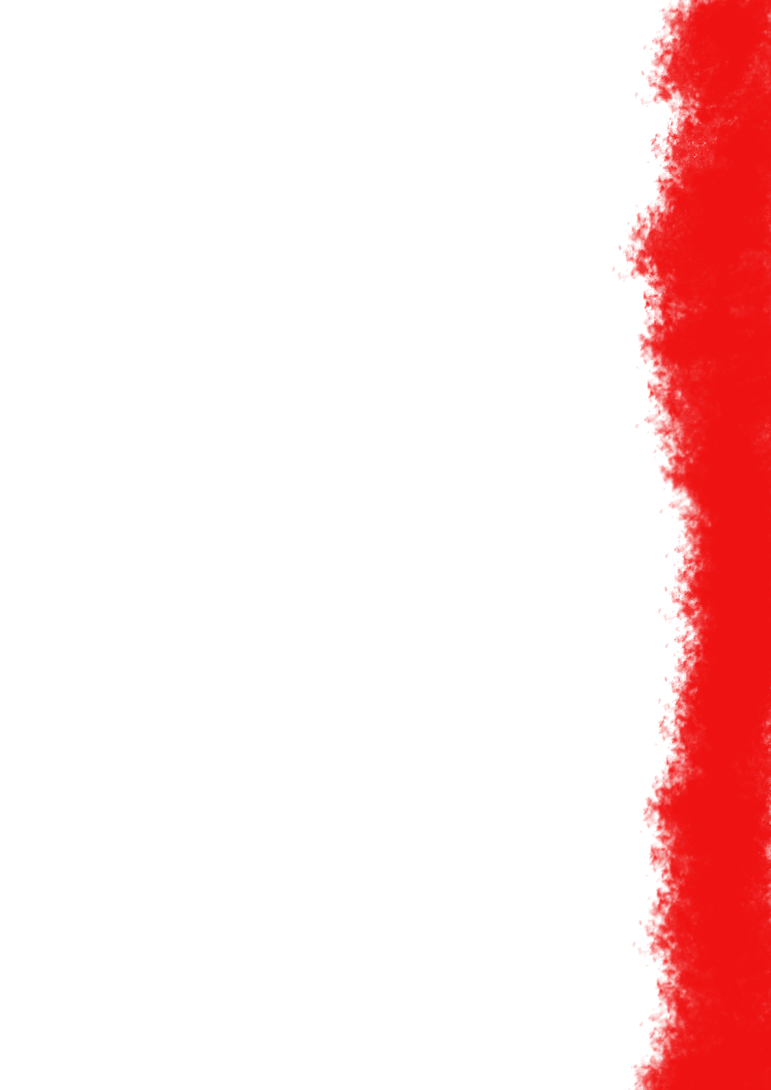
\includegraphics{watermarks/test-a.png}}			% págimas pares
\newwatermark[allpages]{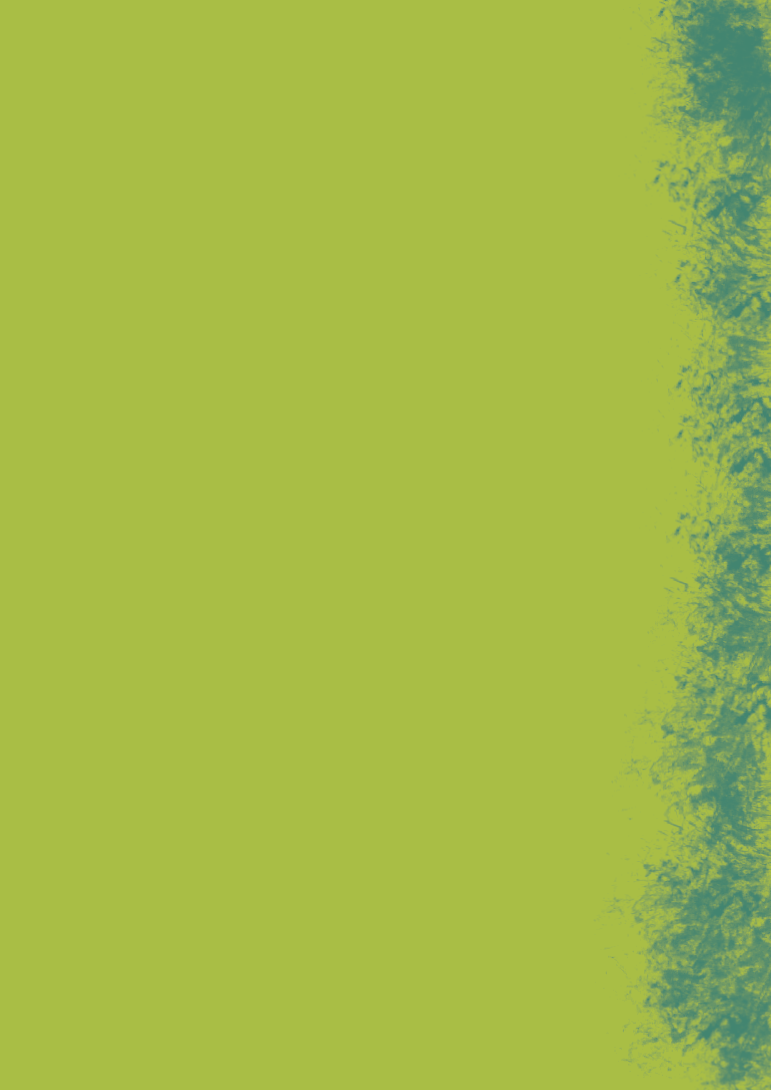
\includegraphics[scale=3.3]{watermarks/test-b.png}}

\pagecolor{cyan!0!magenta!10!yellow!28!black!28!}

\newcommand{\AutorLivro}{Eloar Guazzelli Filho}
\newcommand{\TituloLivro}{Janelas}
\newcommand{\Tema}{Aventuras em contextos imaginários ou realistas; urbanos; rurais; locais; internacionais}
\newcommand{\Genero}{Narrativos: fábulas originais; da literatura universal e da tradição popular}
%\newcommand{\imagemCapa}{./images/PNLD0001-01.png}
\newcommand{\issnppub}{978-65-89705-04-8}
\newcommand{\issnepub}{978-65-89705-06-2}
% \newcommand{\fichacatalografica}{PNLD0001-00.png}
\newcommand{\colaborador}{{Paulo Pompermaier e Renier Silva}}

\begin{document}

\title{\TituloLivro}
\author{\AutorLivro}
\def\authornotes{\colaborador}

\date{}
\maketitle

%\begin{abstract}\addcontentsline{toc}{section}{Carta ao professor}
%\pagebreak

\tableofcontents



\section{Sobre o livro}

%550 caracteres
\paragraph{O livro} \textit{Janelas} apresenta uma narrativa visual pela imaginação de uma menina. Presa em casa devido à pandemia de Covid-19, ela passa a observar a janela de sua casa e vê, através dela, diferentes mundos e universos.
Como toda a narrativa é construída com imagens, o livro 
ofereça inúmeras possibilidades de leitura, pois boa parte de seu sentido é 
construído a partir do olhar e da interpretação do leitor. A participação de quem 
está lendo a obra é fundamental para que a sequência de imagens ganhe sentido e, 
tratando-se de um leitor infantil, as oportunidades para explorar a 
imaginação são inúmeras.

%822 caracteres
\paragraph{Descrição} Sabemos do contexto de pandemia logo nas primeiras páginas do livro, quando observamos um jornal e uma televisão com notícias do vírus e imagens de pessoas mascaradas. A jovem protagonista, sempre de costas para o leitor, passa então a observar a janela de sua casa. Através dela, passam diante de seus olhos (e do leitor) diferentes mundos e universos: em um momento observamos um dragão se movimento por uma cidade medieval; no outro a cidade aparece submersa embaixo da água; rinocerontes voam no céu, ciclopes e duendes passeiam por reinos mágicos. Também observamos a vida na Terra em diferentes contextos: uma caravela navegando; moinhos de vento em campos de trigo; centenas de pinguins no gelo; borboletas e pássaros. Ao final da viagem, os jornais que anunciavam tristezas ao início passam a mostrar desenhos de pessoas felizes e crianças alegres em suas janelas.

%411 caracteres
\paragraph{Competências}
Se todo texto produz sentido, comunica algo, 
um livro-imagem como \textit{A janela} não é um livro sem texto. É uma 
obra cujos textos são visuais, dependentes do movimento criado pela 
sequência das imagens apresentadas ao leitor. As diferentes versões possíveis 
para a história permitem que o pequeno leitor e o mediador da leitura estejam 
no mesmo nível, pois não há um código escrito a ser decifrado. 

A interpretação do código visual 
exige competências que são muito bem desenvolvidas em crianças: 
observação e imaginação e, portanto, permitem debate e troca de ideias durante 
a leitura. A exploração as ilustrações deste livro com seus alunos, contribuirá 
para o enriquecimento do repertório da criança: desde o vocabulário até o 
olhar artístico que também pode ser afinado ao longo do trabalho.


%862 caracteres
\paragraph{Aprofundamento} Este material tem a 
intenção de contribuir para que você consiga desenvolver um trabalho aprofundado 
com esta obra na sala de aula. Você encontrará informações sobre a autora, sobre 
o gênero e sobre os temas trabalhados ao longo do livro. Apresentaremos também 
algumas propostas de trabalho para a sala de aula que você poderá explorar livremente, 
da forma que considerar mais apropriada para os seus estudantes. Para a prática 
da Literacia Familiar, oferecemos um guia que pode ajudar nas orientações aos 
responsáveis pela criança, para incentivar o gosto pela leitura e contribuir para 
que os estudantes desenvolvam em casa habilidades que serão importantes no momento 
da alfabetização. Por fim, você encontrará sugestões de livros, artigos e sites 
selecionados para enriquecer a sua experiência de leitura e, 
consequentemente, a de seus estudantes.



\section{Sobre os autores}

\Image{Foto do autor e ilustrador (Arquivo pessoal; )}{PNLD2022-010-02.png}

%532 caracteres
\paragraph{O autor} Eloar Guazzelli Filho nasceu em Vacaria, Rio Grande do Sul, em 1962. É ilustrador, animador e quadrinista, tendo iniciado sua carreia nos anos 1990 com  publicação de histórias em quadrinhos.
Formado em Artes Plásticas pela Universidade Federal do Rio Grande do Sul (\textsc{ufrgs}), defendeu em 2009 o mestrado sobre o quadrinista Renato Canini na Escola de Comunicações e Artes da Universidade de São Paulo (\textsc{usp}). Recebeu diversas premiações por suas obras e já participou de de exposições em mais de quinze países.


%313 caracteres
\paragraph{Publicações} Em 2010, publicou pela editora Peirópolis uma adaptação em quadrinhos do conto ``Demônios'', de Aluísio Azevedo. Em 2016, ilustrou os livros do \textit{Sítio do Picapau Amarelo} de Monteiro Lobato (Globo Livros). Entre as dezenas de livros que já publicou, constam várias adaptações gráficas de clássicos, como Fernando Pessoa, \textit{A escrava Isaura}, de Bernardo Guimarães, e \textit{Grande sertão: veredas}, de Guimarães Rosa. Também ilustrou livros de autores contemporâneos, como Lygia Fagundes Telles e Fabrício Corsaletti.

%358 caracteres
\paragraph{Currículo} Foi premiado, em 1991, no Yomiuri International Cartoon Contest e no Salão Internacional de Humor de Piracicaba em 1991, 1992 e 1994. Na categoria ``Quadrinhos'', obteve a primeira colocação na 2ª Bienal Internacional de Quadrinhos, no Rio de Janeiro. Em 1994, ganhou o Troféu \textsc{hqm}ix: Desenhista revelação. Recebeu a mesma premiação, em 1999 e em 2000, na categoria livro infantil.
Em 2020, ganhou o Prêmio Vladimir Herzog na categoria ``Prêmio Destaque Vladimir Herzog Continuado''.

\section{Sobre o gênero}

%55 caracteres
\paragraph{O gênero} O gênero deste livro é \textit{narrativo}. 

\Image{O gênero da narrativa proporciona ao leitor uma abertura ao mundo. (Pixabay/Tumisu; CC-BY-2.0)}{PNLD2022-010-07.png}

%596 caracteres
\paragraph{Descrição} 
A narrativa é, essencialmente, um gênero que transmite uma história.
No caso deste livro, a narrativa se dá a partir de imagens, algo fundamental para a educação das crianças. Afinal, as imagens são poderosas formas de comunicação, 
muito presentes na sociedade em que vivemos, desde \textit{outdoors} e manuais de 
instrução até as inúmeras telas com as quais temos contato. Como interpretamos 
imagens o tempo inteiro, não conseguimos perceber com clareza o quanto 
interpretar uma imagem é uma atividade complexa. Ler imagens com competência, 
perceber seus recursos e nuances é parte importante do processo de apreensão, 
leitura e compreensão do mundo e de nossa existência. Antes de ler textos 
verbais, lemos textos visuais e os interpretamos a partir de nossas vivências, 
emoções e percepções.

%603 caracteres
\paragraph{Interação} As crianças são leitores de imagens 
muito competentes: interpretam as expressões nos rostos de seus familiares, 
conseguem identificar objetos apenas pela observação e criar histórias a partir 
de ilustrações em livros com letras que elas ainda não sabem ler. A narrativa imagética 
confere uma liberdade maior ao leitor que está começando a se alfabetizar, pois a narrativa se concentra em uma linguagem que ele consegue ler e construir interpretações de forma 
independente. O leitor infantil e o leitor adulto podem trocar impressões e 
interpretações sobre as imagens livremente, cada um a partir do 
próprio repertório.

%862 caracteres
\paragraph{Competências} 
Para além da narrativa, o livro-imagem 
apresenta às crianças uma linguagem artística complexa. No caso de 
\textit{Janelas}, cada página é uma obra de arte que permite 
uma experiência estética e artística individual. Ela apresenta ao leitor 
uma paisagem ampla, apesar de vista por uma janela, ilustrada com ricos elementos da cultura universal pela técnica de desenho de 
Eloar Guazzelli Filho. Explorar as cores, as formas, o posicionamento dos personagens 
na página, as sugestões imaginativas e fantásticas dos quadros e até mesmo a opinião e os sentimentos das crianças sobre as imagens 
são possibilidades que aprofundarão a leitura, aumentarão o repertório 
e incentivarão o desenvolvimento do vocabulário e da fluidez do discurso. 



\section{Temas}

\subsection{Aventuras em contextos imaginários ou realistas; urbanos; rurais; locais; internacionais}

%136 caracteres
\paragraph{Abordagem} As imagens deste livro levam a criança a uma grande viagem pela imaginação. Em cada página encontramos ricas ilustrações que nos remetem aos mais diversos lugares e pontos da imaginação. Há desenhos para todos os gostos: animais fantásticos, seres mitológicos, cidades abandonadas, criaturas pré-históricas, planetas desconhecidos, cidades futurísticas, astronautas. Independe do ambiente, as composições criam um universo lúdico no qual prevalecem as associações imaginárias pelas quais a criança vai se aventurar.

%206 caracteres
\paragraph{Descrição} O livro oferece uma ótima oportunidade para trabalhar a imaginação e a criatividade ao explorar os elementos imagéticos. Mesmo em um espaço cotidiano e banal, podemos nos aventurar pela imaginação e viver outros mundos, nos quais os fatos mais corriqueiros tornam-se encantados e lúdicos.

%275 caracteres
\paragraph{Competências} Este tema, portanto, 
relaciona-se ao campo da experiência Escuta, fala, pensamento e imaginação 
descrito pela \textsc{bncc}, que tem o intuito de enriquecer o repertório do estudante 
e incentivar que ele exercite formas de comunicação.


\section{Modelagem de aula}
A seguir você encontrará a descrição de uma aula modelo como exemplo 
prático de exploração do livro com estudantes. Esta seção apresentará 
orientações sobre como organizar a sala de aula para receber os 
estudantes, exercitar a interação verbal e prepará-los para o 
momento da leitura.

Em seguida, você encontrará a \textbf{Leitura dialogada}, um 
tópico destinado a te orientar para o momento específico da 
leitura com os estudantes. Por fim, no tópico 
\textbf{Propostas de atividades}, você encontrará ideias 
de práticas que pode explorar com as crianças em sala de 
aula antes, após e durante a leitura. 

Essas atividades podem ser trabalhadas de acordo com a 
disponibilidade do seu cronograma. Fique à vontade para adaptá-las 
da forma que achar melhor para os seus estudantes. Cada turma é única 
e o seu conhecimento prático das características de cada aluno será 
essencial para definir a melhor forma de aplicar essas ideias. 

O objetivo deste manual é oferecer algumas ideias 
e inspirações para um trabalho que pode ser desenvolvido tanto 
a curto, quanto a médio e longo prazo. Sinta-se à vontade para 
personalizar a aula e torná-la sua, aplicando seus conhecimentos, sua 
personalidade e aproveite para fortalecer 
seu vínculo com a turma.


\subsection{Antes de ler}

\BNCC{EI02CG01}
\BNCC{EI02CG02}
\BNCC{EI02CG03}
\BNCC{EI02CG04}
\BNCC{EI02ET02}

%Alterar o nível escolar nesse parágrafo.
Como este trabalho será realizado com crianças da \textbf{Creche 2}, 
que ainda não têm tanta intimidade com o livro enquanto objeto, você terá o 
papel essencial de mediar este contato. 

Nosso objetivo é que os próprios estudantes possam manusear 
e explorar o livro de forma autônoma, mas, para que isto aconteça, você 
pode ajudar a tornar o caminho mais convidativo com atividades que tenham 
intencionalidade educativa. 

A \textsc{bncc} define intencionalidade educativa como ``organização 
e proposição, pelo educador, de experiências que permitam às crianças 
conhecer a si e ao outro e de conhecer e compreender as relações com a 
natureza, com a cultura e com a produção científica, que se traduzem nas 
práticas de cuidados pessoais (alimentar-se, vestir-se, higienizar-se), 
nas brincadeiras, nas experimentações com materiais 
variados, na aproximação com a literatura e no encontro com as 
pessoas''.\footnote{\textsc{bncc}, página 39}

É importante manter essa intencionalidade em mente não apenas na condução 
das atividades propostas neste manual, mas também para aproveitar as 
oportunidades espontâneas de construir conhecimentos que podem surgir durante 
a interação direta com os estudantes.

\begin{enumerate}
%836 caracteres
\item \textbf{O ambiente}\quad Antes de iniciar o trabalho com o livro, é importante que você 
prepare o ambiente para receber a turma. Como o trabalho com o livro terá 
três momentos (antes, durante e depois da leitura), seria interessante que você 
criasse um ambiente para cada etapa. Nas \textbf{Sugestões de referências complementares} 
você encontrará um artigo que discorre sobre a importância da organização da sala 
de aula para a educação infantil, que pode ser um bom guia para a criação desses 
ambientes.
Para o momento antes da leitura, sugerimos uma atividade que estimulará a percepção sobre os diferentes ambientes e desenvolver o contato com a música e diferentes melodias, além de trabalhar os sons corporais e aqueles que se pode fazer com os objetos ao nosso redor. 

%413 caracteres
\item \textbf{Materiais}\quad Rádio ou caixa de som.

%632 caracteres
\item \textbf{Desenvolvimento}\quad Inicialmente, converse com as crianças sobre as janelas e as ocasiões em que elas devem ficar abertas ou fechadas. Ressalte que isso depende do clima que está fazendo, pois se chove, nós fechamos as janelas, mas se faz sol nós abrimos. Em seguida, coloque a música “A janelinha”, do grupo Bob Zoom, e peça para as crianças acompanhem o ritmo da música batendo as mãos e os pés. Quando a música canta “abriu”, elas devem bater com a mão nas pernas; quando a música diz “fechou”, elas devem bater palma com as mãos. É importante insistir para que as crianças consigam entrar no ritmo, pois assim elas desenvolvem sua percepção dos sons e a motricidade, pois trata-se de uma atividade desenvolvimentista.

\item \textbf{Perguntas para avaliar}\quad A turma consegue estabelecer relação entre a janela e o clima que faz? As crianças acompanham o ritmo da música? Conseguem estabelecer relação entre a música e o movimento que faz com o corpo para extrair os sons? 

\end{enumerate}


\subsubsection{A interação verbal} 
Criar situações em que as crianças precisam dialogar diretamente com 
você é uma das práticas mais importantes de Literacia, pois elas estimulam 
o desenvolvimento linguístico, ampliam o vocabulário e reforçam a 
capacidade dos estudantes de compreenderem o que ouvem e se expressarem 
pela fala. O diálogo livre com a criança também reforça sua autoestima, pois 
a faz se sentir ouvida e valorizada pelo adulto, ao vê-lo prestar atenção 
no que ela tem a dizer. Portanto, sempre que possível, reserve um tempo na 
aula apenas para a interação verbal. 

Como esse tipo de interação é espontânea e intimamente atrelada ao 
desenvolvimento de cada estudante, nossas orientações não serão específicas. 
A ideia é que você adapte este momento de acordo com as respostas e os 
repertórios das crianças. É um momento de estreitamento de vínculos e, portanto, 
fique à vontade para ser espontânea e para explorar os tópicos que achar 
mais interessantes para a sua turma.

Inicie as conversas com naturalidade, seguindo os objetos de atenção das crianças. 
Você pode partir de objetos que estejam analisando
para iniciar um assunto e incentivar que se expressem. Ainda que a
criança não fale corretamente, continue interagindo, 
pois a intenção aqui é que a criança perceba que outras pessoas estão respondendo 
à sua comunicação. 

Fique atento a todas as formas de expressão: os gestos, as falas, as 
expressões faciais, para onde olham\ldots{} tudo pode ser explorado durante a conversa. 
Demonstre curiosidade sobre eles, seja um ouvinte entusiasmado e incentive que eles 
conversem entre si. Faça perguntas e construa a resposta junto com as crianças. 

A seguir, algumas dicas que podem contribuir para que a interação verbal 
seja produtiva em sua sala de aula: 

\begin{enumerate}
\item Sente-se no chão e brinque com eles, estabelecendo 
contato visual. Além das pequenas frases que conseguem formar, vocalizações, 
gestos e expressões faciais podem ser boas formas de comunicar.

\item Não se esqueça que a conversa é uma troca e, portanto, 
evite ficar falando sozinho ou desvalorizar as respostas das 
crianças quando não conseguem formular frases completamente articuladas. 
Nunca descarte uma tentativa de comunicação. 

\item Evite utilizar falas negativas que desencorajam o diálogo. 
Se precisar que a turma 
corrija algum comportamento, explique claramente a razão e 
oriente com calma. Incentive positivamente as crianças e 
destaque o motivo de seus elogios. 

\item Aproveite alguns momentos durante a conversa para chamar 
a atenção das crianças para os sons das palavras e das letras que você 
acabou de usar ou que eles pronunciaram.  

\item Fale sempre com as crianças, pois, apesar de alguns estarem começando a falar,
são capazes de compreender muito.

\item Explore possibilidades de interação como apontar e 
nomear objetos, pessoas e animais, imitar a criança ou pedir que 
ela o imite, fazer caretas, reproduzir sons de 
animais para que repitam, ensinar os nomes de partes do corpo, 
entre outras atitudes que estimulem a comunicação com a criança. 

\item Muitas dessas dicas poderão ser aproveitadas pela 
família durante a prática da Literacia Familiar. Portanto, 
se achar necessário, compartilhe algumas destas orientações 
com as famílias dos estudantes.
\end{enumerate}


\subsection{A leitura dialogada}
Este é o momento em que será realizada a leitura propriamente dita. 
Se possível, crie um \textit{cantinho da leitura} em sua sala de aula. Um 
ambiente confortável, de preferência em que todos se sentem no chão ou 
em pufes para que consigam enxergar as ilustrações do livro que está 
sendo lido e interagir com facilidade. Se houver possibilidade, mantenha 
sempre os livros da turma em uma altura da estante que permita fácil 
acesso para os estudantes ou guarde os livros em uma caixa que as crianças 
possam mexer com autonomia. É importante que elas tenham autonomia para 
acessar os livros e se sintam à vontade para pegá-los sempre que quiserem. 

\Image{É importante que o cantinho da leitura proporcione autonomia para as crianças. (Elza Fiúza/ Agência Brasil; CC BY-NC 2.0)}{PNLD2022-010-08.png}

Outra possibilidade de ambiente para esta leitura, se a escola permitir, 
é efetuar essa leitura ao ar livre, embaixo de uma árvore, onde as crianças 
possam ouvir os sons dos pássaros e sentir o cheiro da grama. Sair da sala 
de aula pode oferecer um ótimo leque de experiências aos seus estudantes e 
reforçar a conexão entre a natureza do livro e a realidade.  

Reserve uma boa parte da aula para o momento da leitura com os estudantes, 
pois é importante que esse momento aconteça sem pressa. O objetivo da 
leitura dialogada é que seja uma leitura em bate-papo. A criança deve 
assumir um papel ativo na leitura, mesmo que ainda não seja capaz de 
ler sozinha. Além de promover o gosto pela leitura, esta prática estimula 
o desenvolvimento da linguagem, enriquece o vocabulário e 
aumenta o conhecimento de mundo.

%Especificar o livro.
No caso de \textit{Janelas} o diálogo durante a leitura é 
ainda mais importante, considerando que não há texto verbal e, 
portanto, a narrativa se apoiará principalmente na sua interação com as crianças. 
Você deve interagir com elas durante toda a 
leitura, fazendo perguntas e partindo de detalhes do livro para 
levantar novas questões.

A seguir, algumas orientações para aproveitar este momento: 

\begin{enumerate}
%177 caracteres
\item \textbf{Contexto}\quad Esta proposta tem o objetivo de estimular a imaginação e a criatividade da criança a partir de imagens ou temas presentes no livro.  
 
\item \textbf{Como começar}\quad Tente organizar as crianças em roda. O professor, então, folheia o livro página a página, mostrando as imagens de janelas que estão em \textit{Janelas}. Enquanto isso, é interessante questionas os alunos sobre o que cada imagem está representando.

%230 caracteres
\item \textbf{Manuseio}\quad Deixe que as crianças manuseiem o livro 
e explore com elas todos os elementos que o compõem. Mostre o que é a 
capa e onde estão as páginas.

%495 caracteres
\item \textbf{Diálogo}\quad O livro possui imagens com grande distância, como a de um centro municipal com prédios, pedestres e carros, e, em outra página, imagens com grandes proximidades, como o olho de um animal. É interessante que o professor chame a atenção das crianças para as imagens mostradas, fale sobre essas diferenças de perspectiva e questione o que elas enxergam. Pode-se fazer perguntas que instiguem as crianças a falar sobre as imagens, como:

\begin{itemize}
\item Quais as diferenças de uma imagem/janela para outra?
\item Qual está mais perto? E mais longe?
\item O que vocês imaginam com essa imagem?
\end{itemize}

Incentive que falem para responder.
Abra a conversa para que todos possam participar. Se os estudantes não 
conseguirem responder, explique e contextualize sua
resposta.

%346 caracteres
\item \textbf{Escuta}\quad Elogie atitudes positivas, como 
tentar tomar o papel central na conversa sobre as imagens. Se os estudantes tentarem 
tomar o seu lugar e começar a falar sobre alguma ilustração, valorize e escute com atenção o que estiverem falando. Mas não 
force a leitura. Se as crianças estiverem cansadas, faça outra atividade 
e retorne depois. 

%935 caracteres
\item \textbf{Leitura}\quad Faça perguntas e comentários que aumentem o 
interesse e aticem a curiosidade das crianças sobre as ilustrações e as possibilidades de narração com o encadeamento das imagens. Faça 
perguntas ou comentários como: 

\begin{itemize}
\item O que você acha que aconteceu depois disso?
\item Qual a relação entre essas duas figuras?
\item Você prefere a imagem de qual janela?
\end{itemize}

Não tenha pressa em passar as páginas. Deixe que os estudantes 
observem as ilustrações, dê tempo para que construam suas narrativas e ideias 
a partir das ilustrações apresentadas na página.

Ao explorar o texto visual, dê emoção 
à leitura. Invente diálogos entre os personagens, crie uma voz para 
cada uma, capriche nas expressões faciais e imite os sons dos animais e objetos que aparecem.
Deixe-se guiar pela atenção das crianças, mas se perceber que 
elas estão dispersas ou saltando aleatoriamente as páginas, ajude-as 
a retornar à narrativa. Crie um ambiente amigável onde a criança 
se sinta à vontade para fazer perguntas e comentários durante a leitura.


%382 caracteres
\item \textbf{Interação}\quad Nomeie os elementos das ilustrações 
do livro, apontando para elas com o dedo. Destaque os sons de algumas 
palavras mais difíceis. Interrompa a leitura em alguns momentos e peça que 
os estudantes falem sobre o que estão pensando ao observar as ilustrações do livro.
Se possível, explore outras ordens do livro, abrindo-o aleatoriamente ou começando do fim.
Você pode criar uma narrativa diferente para as diferentes formas de encadear as ilustrações.
Ao final do livro, para aprofundar ainda mais a interação, você pode pedir para que as crianças escolham uma dessas janelas e representem o que elas veem. Pode-se utilizar massinha de modelar para fazer a representação, explorando o tato e a forma. Mas, na impossibilidade de usar esse material, as crianças podem desenhar o que elas observam da janela escolhida. Em seguida, eles podem comparar suas produções com os demais colegas.  

\Image{As crianças podem desenhar ou usar massinha de modelar para representar o que veem da janela. (PxHere; CC0)}{PNLD2022-010-09.png}

\item \textbf{Perguntas para avaliar}\quad As crianças conseguem estabelecer as diferenças entre as imagens do livro? E as diferenças entre as janelas de suas casas? As crianças representam imagens que encontraram no livro?  

\end{enumerate}


\subsection{Proposta de atividade}

\BNCC{EI02TS02}
\BNCC{EI02CG05}
\BNCC{EI02EF06}
\BNCC{EI02E003}
\BNCC{EI02E006}


\begin{enumerate}
%700 caracteres
\item \textbf{Contexto}\quad Após a leitura dialogada, é hora de criar 
atividades que proporcionem aos estudantes experiências novas a partir do livro
que acabaram de conhecer.
Esta proposta tem o objetivo de estimular a criatividade com base em imagens prévias. O intuito é que as crianças possam criar juntas, estimulando a troca entre os pares.

\item \textbf{Materiais}\quad Caixa de papelão; tesoura; papel crepom; E.V.A; cola.

%950 caracteres
\item \textbf{A atividade}\quad Monte, junto com as crianças, uma janela de papelão que possa ser posicionada em alguma parte da sala de aula. Essa janela pode ter o nome de “Janela da imaginação”. A proposta é que todos possam ajudar a enfeitar essa janela, de acordo com as suas possibilidades e habilidades manuais. Caso necessário, o educador pode realizar a etapa mais difícil da confecção da janela. Basta cortar uma caixa de papelão, formando uma borda que poderá ser enfeitada com bolinhas, florzinhas e outras figuras ou objetos criados pelos alunos. Com a caixa posicionada em uma mesa e estabilizada com fita crepe, as crianças, em grupos de três, posicionam-se próximas à janela e contam uma história breve de sua imaginação ou memória, criando um clima de fantasia, em que a janela da imaginação permite a todos criar e/ou contar suas histórias. É importante que o professor auxilie os grupos, dando sugestões e estipulando um tempo para que todos no grupo possam participar. Pode ser uma história que o professor já contou, ou uma historinha que já viram na TV ou no teatro, e até mesmo uma história inventada.  

\Image{Ideias para decorar a janela da imaginação. (Public domain pictures; Domínio público)}{PNLD2022-010-10.png}

%550 caracteres
\item \textbf{Interação}\quad Essa atividade proporciona aos estudantes a possibilidade de fazer relações entre o livro e sua vida cotidiana, pois vão trazer ao ambiente da ``janela da imaginação'' coisas que eles viveram, viram ou ouviram. Quando as crianças propuserem suas ideias, interaja com o pensado e apresentado pelas crianças, fazendo perguntas que as auxiliem a desenvolver o pensamento iniciado.
Relacione seus gestos e palavras às imagens que aparecem no livro, fazendo perguntas relacionadas ao que a criança contou, incentivando-as a se abrirem e estabelecerem conexões com as imagens exploradas durante a leitura.

\item \textbf{Perguntas para avaliar}\quad As crianças conseguem se comunicar entre si e entrar em acordo? Elas conseguem devolver uma história que faça sentido para quem assiste? As sugestões ajudam a criança a desenvolver a história?
\end{enumerate}


\section{Literacia familiar}
O \textsc{pna} dá destaque especial para a importância do envolvimento da família 
no processo pedagógico nesta faixa etária e denomina Literacia Familiar o conjunto 
de experiências e práticas relacionadas à linguagem (oral, escrita ou lida) vivenciadas 
com os cuidadores. 

Essas estratégias podem começar a ser colocadas em prática desde a 
gestação e continuar até o final da adolescência. São práticas simples e divertidas 
que estimulam o desenvolvimento de quatro atividades fundamentais: ouvir, falar, 
ler e escrever que criam momentos de afeto e interação para a família. 

Para que esse trabalho conjunto entre escola e família funcione, é 
fundamental que a escola esteja em constante diálogo com os responsáveis e 
você consiga orientá-los. Um grupo em aplicativos de mensagens instantâneas ou um 
grupo de e-mails são saídas viáveis para que a comunicação se estabeleça e pode ser 
uma forma útil das famílias compartilharem suas vivências e trocarem sugestões 
de abordagens, sempre contando com a sua mediação. 

Com o objetivo de incentivar 
a prática da \textit{literacia familiar}, se possível, organize um rodízio entre os familiares 
das crianças para emprestar o livro da biblioteca da turma. Neste caso, crie um caderno 
de registro e estabeleça períodos para cada família ficar com o livro. É importante 
que os familiares compreendam a seriedade deste compromisso, pois o livro pertence 
ao acervo da sala e, portanto, deve ser bem cuidado e devolvido na data acordada. 

Se não for possível garantir o acesso direto dos cuidadores da criança ao livro, 
grave um vídeo direcionado a eles, contando a história e apresentando algumas 
das ilustrações. O importante é que os familiares saibam com clareza qual livro 
está sendo trabalhado, a história contada e se sinta seguro para explorar as temáticas 
do livro com a criança. Orientações claras e a manutenção do canal de comunicação com 
os responsáveis é essencial para que eles se sintam seguros e à vontade para fazer perguntas 
se tiverem dúvidas. 

Neste manual, você encontrará algumas práticas que podem ser 
recomendadas aos familiares para ajudá-los a expandir e aprofundar o trabalho 
que você iniciou em sala de aula.


\subsection{Importância da leitura}
Na escola, aprendemos a ler letras, mas é importante ter em mente que nós 
lemos o mundo desde muito pequenos: “lemos” os animais que passam pelos nossos 
quintais, a expressão no rosto dos nossos familiares, as cores que pintam o céu 
em um fim de tarde. 

Vamos aprendendo, ao longo da vida, a interpretar acontecimentos 
e sons que escutamos e a utilizá-los para nossa comunicação. Aprender a ler textos e 
escrevê-los expande a nossa leitura do mundo, pois permite que sejamos capazes de 
interpretar um código e experimentar, a partir dele, novas experiências e conhecimentos. 

O simples contato com os livros já permite um leque grande de sensações: 
sentimos as texturas, as formas, vemos as cores do livro, escutamos o som da página 
virando e o som da voz do narrador, se a história estiver sendo lida em voz alta. Para uma 
criança pequena, são experiências que podem contribuir diretamente com o desenvolvimento psicomotor 
e cognitivo. 

Nosso papel, enquanto mediadores de leitura, é contribuir para que essas 
sensações sejam associadas a momentos positivos, de construção de 
conhecimento e exercício de imaginação. 

Com os livros, podemos conhecer mais da história humana, descobrir informações 
novas sobre sociedades diferentes da nossa, imaginar situações e contextos inéditos 
para nós e aumentar o nosso repertório. São por meio deles que melhoramos nossa 
capacidade de interpretação, de expressão, de análise e senso crítico. Boas habilidades 
leitoras podem contribuir para o desenvolvimento de um estudante em todas as outras 
disciplinas, pois exercem influência direta na forma como absorvemos e 
construímos conhecimento.


\subsection{O papel da família na formação do leitor}
A família é peça fundamental na formação do leitor, pois é ela quem primeiro 
ensina a criança a ler. Não apenas os textos escritos, mas a ler o mundo, a 
interpretar os estímulos que a cercam, a construir seu próprio vocabulário e a 
comunicar seus pensamentos e necessidades. Na fase em que estão, os bebês 
absorvem o conhecimento com voracidade e tentam aprender a se comunicar. 

O universo das letras é muito presente na vida das crianças antes mesmo de sua 
entrada na escola. Aparece nas histórias e ilustrações do livro que o cuidador 
lê ao colocá-la para dormir, nas situações em que vê os responsáveis se comunicarem 
pela escrita ou nos textos que podem permear seu cotidiano (nos outdoors, na 
televisão, no celular, manuais de instrução entre outros). 

Os familiares têm, 
portanto, uma ótima oportunidade de apresentar a leitura com leveza, de forma 
prazerosa, associado ao contexto em que a criança vive e à momentos de diversão. 
Você poderá orientar os pais nesta tarefa, ensinando-os com este guia a aproveitar 
as oportunidades para trabalhar a Literacia com a criança.


\subsubsection{Práticas de literacia familiar} 

São muitas as experiências que a prática da \textit{literacia familiar} 
pode oferecer às crianças. A seguir, explicamos cada uma delas para que você possa, 
se achar necessário, compartilhar com os responsáveis enquanto estiver orientando-os: 

\paragraph{Interação verbal} Aumentar a quantidade de conversas com as 
crianças, fazendo perguntas para incentivar o diálogo.

\paragraph{Leitura dialogada} Interagir com a criança durante a leitura 
em voz alta, criar expectativa sobre o livro, chamar a atenção para detalhes 
das ilustrações e comentar o enredo.

\paragraph{Narração de histórias} Interagir com a criança enquanto 
estiver narrando uma história, por exemplo, incluindo-a na ação, utilizando 
marionetes ou permitindo que ela complete a narrativa.

\paragraph{Contatos com a escrita} Apresentar as letras para as 
crianças, incentivar que tentem escrever ou ler, ajudá-los a desenhar letras, 
entre outras formas de incentivar o contato com as palavras.

\paragraph{Atividades diversas} Qualquer atividade com a criança 
pode ser utilizada para contribuir para a alfabetização. Jogos, brincadeiras, 
instrumentos musicais, canto, dança, passeios e viagens oferecem boas 
oportunidades de aprendizado.

\paragraph{Motivação} Atitudes que motivem as crianças à envolver-se com 
o mundo da leitura e da escrita.

\subsection{Exercitando a literacia familiar}

\BNCC{EI02EO03}
\BNCC{EI02EO04}
\BNCC{EI02CG02}
\BNCC{EI02EF01}
\BNCC{EI02EF06}
\BNCC{EI02ET02}
\BNCC{EI02ET04}

\begin{enumerate}
%700 caracteres
\item \textbf{Como começar}\quad Para iniciar o contato da família com o livro, na interação com a criança, pode-se solicitar aos pais que explorem o tema das janelas com as crianças, seguindo um pouco a atividade proposta na pré-leitura.
Solicite aos familiares que conversem com as crianças sobre o que elas veem quando abrem a janela de suas casas. Os pais, nesse processo, podem estimular a criatividade da criança, como perguntas como: o que elas gostariam de ver de suas janelas? Elas preferem o dia ensolarado ou mais ameno ao olharem pela janela? Elas já pararam para observar pelas janelas? O que elas sentem com isso? Têm vontade de sair para a rua, ou gostam de observar o que acontece lá fora?
Em seguida, os pais podem auxiliar as crianças a fazer um desenho que represente essa visão da janela, valendo aqui a imaginação: tanto o que veem pela janela no quotidiano, como o que gostariam de ver etc.


%650 caracteres
\item \textbf{Leitura}\quad A família pode continuar explorando os temas apresentados pelo livro em relação às janelas que as suas crianças observam.
Os familiares podem explorar 
elementos do cotidiano que se relacionam à história e indicar a conexão 
entre o que viram na ilustração e a realidade. A história de \textit{Janelas}
se passa em um ambiente fechado que, pela imaginação, se faz infinito.
Os familiares podem aproveitar este fato 
para comparar as diferentes visões que cada janela de sua casa tem.
Pode-se ressaltar as semelhanças e diferenças entre a perspectiva vista de cada janela, apontando elementos interessantes e comparando a janela à imaginação, pela qual passam diferentes imagens a cada momento.
Oriente os pais a mostrar as 
árvores, pássaros, prédios, telhados e pessoas que podem ser vistas da janela, relacionando-os à visão criativa que podem imprimir sobre cada elemento cotidiano.
Assim a atividade da escolinha ganha sentido na vida cotidiana das crianças.


%1073 caracteres
\item \textbf{Instrução}\quad Informe aos pais sobre a estrutura do livro e as principais competências desenvolvidas em sala de aula, ressaltando a importância da imaginação e sua relação com os gestos corporais, como desenvolvido na atividade de pré-leitura.
Oriente-os a, quando possível, a folhear o livro com a criança e criar novas narrativas para as imagens.
Desta forma as crianças terão contato com a mesma imagem de duas formas distintas, através da mediação em sala de aula e em família. 
Mesmo pequenas, as crianças conseguem perceber a diferença entre 
as formas de contar, e elementos da narração em casa podem ajudá-la a compreender 
sentidos e perceber detalhes que não foram explorados em sala de aula.
Outra opção é entregar o livro para a criança e pedir que ela tente se lembrar
do que foi falado em sala de aula, quais elementos foram destacados e enfatizados pelo educador e pelos colegas. Mesmo que a memória não pareça 
completa para o adulto, é importante que ele ouça com atenção e 
valorize todas as tentativas da criança. Afinal, ao tentar recontar, 
ela manipulará o livro, treinará a coordenação motora, conhecerá as texturas 
do objeto e poderá imitar a forma como o adulto 
conta a história, treinando a fala. 
Na impossibilidade de ter o livro em casa, é possível solicitar aos familiares que leiam e/ou assistam histórias com as crianças, pois, isso estimula a criatividade e a afetividade entre os pares. Como é um livro amplo, com ilustrações que remetem aos mais diversos universos e elementos, as atividades desenvolvidas no livro também podem ser levadas a outros suportes e outras narrações. 
\end{enumerate}

 
\section{Sugestões de referências complementares}

\subsection{Livros} 

\begin{itemize}
\item \textsc{lins}, Guto. \textit{Livro infantil? projeto gráfico, metodologia, subjetividade}. São Paulo: Rosari, 2002.

Livro que aborda a importância das escolhas visuais (ilustração, projeto gráfico, lettering) na literatura infantil.  

\item \textsc{hunt}, Peter. \textit{Crítica, teoria e literatura infantil}. São Paulo: Cosac Naify, 2010.

Livro sobre crítica de literatura infantil que contêm definições de livro ilustrado e livro imagem. 
\end{itemize}

\subsection{Artigos}

\begin{itemize}
\item \textsc{sardelich}, Maria Emilia. Leitura de Imagens, Cultura Visual e Prática Educativa. 
In: Cadernos de Pesquisa. V.36, n.128, p.451-472, mai/ago.2006. Disponível em: \url{https://www.scielo.br/pdf/cp/v36n128/v36n128a09}. 
Acesso em 29 abr 2021. 

Artigo acadêmico que discorre sobre a importância de trabalhar cultura 
visual na educação na sociedade contemporânea. 

\item \textsc{pranke}, Marha Elfrida. Organização dos espaços da sala de aula na Educação Infantil. Disponível em: \url{http://centraldeinteligenciaacademica.blogspot.com/2016/04/organizacao-dos-espacos-da-sala-de-aula.html}. Acesso em 04 mai 2021. 

Artigo acadêmico que discorre sobre a importância da rotina e de criar ambientes dentro da sala de aula na Educação Infantil.  
\end{itemize}

\subsection{\textit{Sites}}

\begin{itemize}
\item Vídeos “Conta pra mim” no site do PNA. Disponível em: \url{http://alfabetizacao.mec.gov.br/contapramim}. 
Acesso em 13 abr. de 2021.

Página do \textsc{mec} com vídeos sobre leitura dialogada que visam incentivar a Literacia Familiar. Muitas das 
técnicas, explicações e materiais disponíveis nessa página podem ser utilizados em aula, mas o site também 
pode ser uma ótima indicação para ajudar a direcionar os cuidadores dos estudantes a praticar 
a literacia familiar e leitura dialogada.

\item Vídeo “Livros de imagem: como utilizar com as crianças?” do canal Conta Outra. Disponível em Youtube. 
Acesso em 14 abr. 2021. 

Neste vídeo, a pedagoga Bel explica o que são livros de imagem e faz sugestões para mediar a leitura com 
crianças. Se você achar conveniente, esse vídeo pode ser recomendado aos familiares da criança 
para inspirá-los na leitura dialogada. 
\end{itemize}

\section{Bibliografia comentada}

\subsection{Livros}

\begin{itemize}
\item \textsc{brasil}. Ministério da Educação. Base Nacional Comum Curricular. Brasília, 2018.

Consultar a \textsc{bncc} é essencial para criar atividades para a turma. Além de especificar 
quais habilidades precisam ser desenvolvidas em cada ano, é fonte de informações sobre 
o processo de aprendizagem infantil. 

\item \textsc{brasil}. Ministério da Educação. Secretaria de Alfabetização. Conta pra mim: Guia de Literacia Familiar. 
Brasília: \textsc{mec, sealf}, 2019. Disponível em: \url{http://alfabetizacao.mec.gov.br/images/conta-pra-mim/conta-pra-mim-literacia.pdf}.

Este guia é voltado aos pais e oferece explicações em uma linguagem bastante acessível e detalhada as práticas de Literacia Familiar, 
como praticar leitura dialogada, como narrar histórias, como exercitar interação oral, formas de proporcionar contatos com a escrita à criança etc. 
 
\item \textsc{brasil}. Ministério da Educação. Secretaria de Alfabetização. PNA Política Nacional de Alfabetização/Secretaria 
de Alfabetização. Brasília: \textsc{mec, sealf}, 2019.

Um guia fundamental para trabalhar pré-alfabetização e alfabetização de estudantes, que ressalta a importância da Literacia e da Numeracia. 

\item \textsc{van der linden}, Sophie. Para ler o livro ilustrado. São Paulo: Cosac Naify, 2011.

Livro sobre as particularidades do livro ilustrado, que apresenta as diferenças entre o livro ilustrado e o livro com ilustração. 
\end{itemize}

\subsection{Artigos}

\begin{itemize}
\item \textsc{costa}, A. C. C.; \textsc{santos neto}, J. A.; \textsc{bortolin}, S; \textsc{pereira}, Ana Paula. O livro de imagem e a mediação na escola. 
In \textsc{vii secin}, Universidade de Londrina. Disponível em \url{http://www.uel.br/eventos/cinf/index.php/secin2017/secin2107/paper/viewFile/445/296}. 
Acesso em 29 abr 2021
. 
Esse artigo reflete sobre a importância de se apresentar livros de imagem para os estudantes na escola para que as crianças aprendam a ler imagens. 

\item \textsc{nannini}, P. B. R.; \textsc{medeiros}, J. P. S.; \textsc{ribeiro}, J. M. Leitura em cena: Vivências em sala de aula com livro de imagens. 
Literartes, n. 3, p. 82-101, 2014. DOI: 10.11606/issn.2316-9826.literartes.2014.89204. 
Disponível em \url{https://www.revistas.usp.br/literartes/article/view/89204/92115}. Acesso em 29 abr. 2021. 

Artigo acadêmico sobre um trabalho utilizando o mesmo livro de imagem com crianças da educação infantil e ensino médio. 
É uma forma interessante de perceber que a leitura de imagens pode ser explorada com qualquer faixa etária. 
\end{itemize}

% \includepdf[nup=2x2, 					% grid
			% offset=-15mm -5mm, 		% posição
			% scale=.8, 				% tamanho da página
            % delta=4mm 4mm, 			
            % frame,
            % pages={1-4}]{pdfs/PNLD2022-010_MIOLO.pdf}

\end{document}
